\documentclass{article}

\usepackage{pdfpages}
\usepackage[nottoc]{tocbibind}
\usepackage{color}
\usepackage{wrapfig}
\usepackage{graphicx}
\usepackage{subcaption}
\graphicspath{ {../plots/} }
\usepackage{tikz}
\usetikzlibrary{calc,positioning,arrows}
\usepackage{amsmath,amsthm}


\iffalse
\newcommand{\comment}[1]{\textit{\textcolor{blue}{/* #1 */} }}
\fi
\newcommand{\todo}[1]{\textit{\textcolor{red}{// TODO: #1} }}
\newcommand{\draft}[1]{\textit{\textcolor{olive}{#1} }}
\newcommand{\code}[1]{\texttt{#1}}


\theoremstyle{plain}
\newtheorem{thm}{Theorem}[section]
\newtheorem{lem}[thm]{Lemma}
\newtheorem{prop}[thm]{Proposition}
\newtheorem*{cor}{Corollary}

\theoremstyle{definition}
\newtheorem{defn}{Definition}[section]
\newtheorem{conj}{Conjecture}[section]
\newtheorem{exmp}{Example}[section]

\theoremstyle{remark}
\newtheorem*{rem}{Remark}
\newtheorem*{note}{Note}


\begin{document}
\iffalse
\fi
\newcommand{\seqnode}[3][]{ 
  \node[#1] (#2) {#3};
  \node[below of=#2, node distance=5cm] (#2_g) {};
  \draw (#2) -- (#2_g);
}
\newcommand{\hseqnode}[3][]{ 
  \node[#1] (#2) {#3};
  \node[below of=#2, node distance=5cm] (#2_g) {};
}
\newcommand{\msg}[5][above]{
  \draw[->] ($(#2)!#4!(#2_g)$) -- node[#1,scale=0.75,midway]{#5} ($(#3)!#4+0.04!(#3_g)$);
}
\newcommand{\fetch}[4]{
  \draw[-] ($(#1)!#3-0.04!(#1_g)$) -- node[above,scale=0.75,midway]{#4} ($(#2)!#3!(#2_g)$);
  \draw[->] ($(#2)!#3!(#2_g)$) -- node[above,scale=0.75,midway]{} ($(#1)!#3+0.04!(#1_g)$);
}

\tableofcontents
\pagebreak
\section{Introduction}
\todo{What are we doing. Why are we doing this}

\pagebreak
\section{Background}
\todo{Fairly detailed section on rdma / ibverbs. Explain all verbs.}


\pagebreak
\section{Related Work}

\todo{Overview of related papers. Include different benchmark papers}

\todo{Maybe also include systems using rdma protocols. Compare to our findings. Should they have used other connection? 
Maybe add this after the protocols section?}

\pagebreak
\section{Performance Model}\label{sec:perf-model} \label{sec:model}

We looked at what is involved in an RDMA transmission in Figure \ref{fig:seq-sndrcv}.\todo{Figure in RDMA background}
Trying to closely model this however gives us a far too complex model, with a lot of parameters that are hard to assess,
especially if we start to look at more complex protocols. 

We simplify our model by using a modified \emph{LogGP model}~\cite{}. The LogGP model was designed to model point to point
communication with variable message sizes. \todo{Intro to LogGP}


The LogGP model was designed for classical IP based messaging and did not take into account any offloading to the NIC. We 
can however integrate the heavy offloading happening in RDMA by splitting the offset $o$ into multiple offsets for each
of the components. This leaves us with the following parameters.


\begin{itemize}
  \item $L$: an upper bound on the Latency, incurred in sending a message from the senders NIC to the receivers NIC
  \item $G$: the Gap per byte for long messages. For our purposes this is the time of sending a single byte given the 
    maximum bandwidth of our link.
  \item $g$: he gap, defined as the minimum time interval between consecutive message transmissions.
  \item $P$: the number of processes (or servers).
  \item $o_{snd}$: the \emph{send overhead}, defined as the length of time that a processor is engaged in sending each message.
  \item $o_{nsnd}$: the \emph{send NIC overhead}, defined as the length of time that a NIC is engaged in sending each message.
  \item $o_{rcv}$: the \emph{receive overhead}, defined as the length of time that a processor is engaged in receiving each message.
  \item $o_{nrcv}$: the \emph{receive NIC overhead}, defined as the length of time that a NIC is engaged in receiving each message.
  \item $g_{rcv}$: the \emph{receive gap}, defined as the time interval between the receiving processor having received a message 
    and it being ready to process the next message. One example of this gap would be preparing a new receive buffer.
\end{itemize}

\begin{figure}[!ht]
\begin{center}
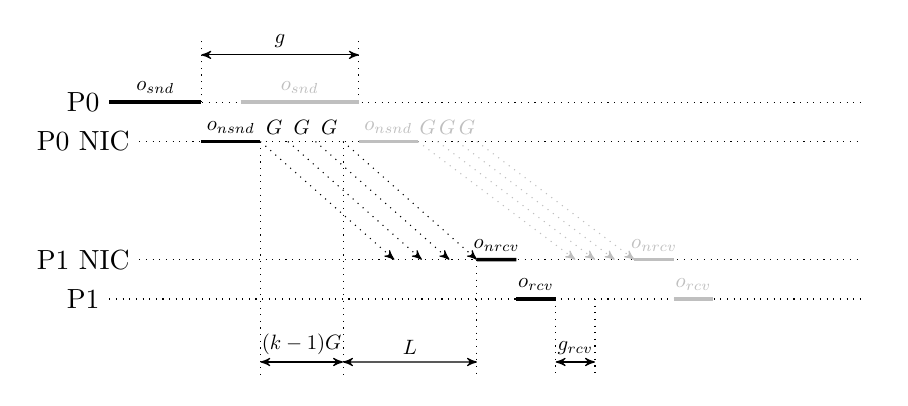
\begin{tikzpicture}[node distance=1cm,auto,>=stealth']
  \node[] (p0) {P0};
  \node[right of=p0, node distance=10cm] (p0_g) {};
  \draw[dotted] (p0) -- (p0_g);

  \node[below of=p0, node distance=0.5cm] (p0_nic) {P0 NIC};
  \node[right of=p0_nic, node distance=10cm] (p0_nic_g) {};
  \draw[dotted] (p0_nic) -- (p0_nic_g);

  \node[below of=p0_nic, node distance=1.5cm] (p1_nic) {P1 NIC};
  \node[right of=p1_nic, node distance=10cm] (p1_nic_g) {};
  \draw[dotted] (p1_nic) -- (p1_nic_g);

  \node[below of=p1_nic, node distance=0.5cm] (p1) {P1};
  \node[right of=p1, node distance=10cm] (p1_g) {};
  \draw[dotted] (p1) -- (p1_g);
  

  %%%%

  \draw[very thick] (p0) --node[above,scale=0.75,midway]{$o_{snd}$} ($(p0)!0.15!(p0_g)$);
  \draw[very thick] ($(p0_nic)!0.15!(p0_nic_g)$) --node[above,scale=0.75,midway]{$o_{nsnd}$} ($(p0_nic)!0.225!(p0_nic_g)$);


  \path[] ($(p0_nic)!0.225!(p0_nic_g)$) --node[above,scale=0.75,midway]{$G$} ($(p0_nic)!0.26!(p0_nic_g)$);
  \draw[dotted, ->] ($(p0_nic)!0.225!(p0_nic_g)$) -- ($(p1_nic)!0.395!(p1_nic_g)$);

  \path[] ($(p0_nic)!0.26!(p0_nic_g)$) --node[above,scale=0.75,midway]{$G$} ($(p0_nic)!0.295!(p0_nic_g)$);
  \draw[dotted, ->] ($(p0_nic)!0.26!(p0_nic_g)$) -- ($(p1_nic)!0.43!(p1_nic_g)$);

  \path[] ($(p0_nic)!0.295!(p0_nic_g)$) --node[above,scale=0.75,midway]{$G$} ($(p0_nic)!0.33!(p0_nic_g)$);
  \draw[dotted, ->] ($(p0_nic)!0.295!(p0_nic_g)$) -- ($(p1_nic)!0.465!(p1_nic_g)$);

  \draw[dotted, ->] ($(p0_nic)!0.33!(p0_nic_g)$) -- ($(p1_nic)!0.5!(p1_nic_g)$);


  \draw[very thick] ($(p1_nic)!0.5!(p1_nic_g)$) --node[above,scale=0.75,midway]{$o_{nrcv}$} ($(p1_nic)!0.55!(p1_nic_g)$);
  \draw[very thick] ($(p1)!0.55!(p1_g)$) --node[above,scale=0.75,midway]{$o_{rcv}$} ($(p1)!0.6!(p1_g)$);
    
  %%%%

  \draw[dotted] ($(p0_nic)!0.225!(p0_nic_g)$) -- ($(p0_nic)!0.225!(p0_nic_g)+(0,-3)$);
  \draw[dotted] ($(p0_nic)!0.330!(p0_nic_g)$) -- ($(p0_nic)!0.330!(p0_nic_g)+(0,-3)$);
  \draw[<->] ($(p0_nic)!0.225!(p0_nic_g)+(0,-2.8)$) --node[above,scale=0.75,midway]{$(k-1)G$} ($(p0_nic)!0.330!(p0_nic_g)+(0,-2.8)$);

  \draw[dotted] ($(p1_nic)!0.5!(p1_nic_g)$) -- ($(p1_nic)!0.5!(p1_nic_g)+(0,-1.5)$);
  \draw[<->] ($(p0_nic)!0.330!(p0_nic_g)+(0,-2.8)$) --node[above,scale=0.75,midway]{$L$} ($(p1_nic)!0.5!(p1_nic_g)+(0,-1.3)$);

  \draw[dotted] ($(p1)!0.6!(p1_g)$) -- ($(p1)!0.6!(p1_g)+(0,-1)$);
  \draw[dotted] ($(p1)!0.65!(p1_g)$) -- ($(p1)!0.65!(p1_g)+(0,-1)$);
  \draw[<->] ($(p1)!0.6!(p1_g)+(0,-.8)$) --node[above,scale=0.75,midway]{$g_{rcv}$} ($(p1)!0.65!(p1_g)+(0,-.8)$);

  \draw[dotted] ($(p0)!0.15!(p0_g)$) -- ($(p0)!0.15!(p0_g)+(0,.8)$);
  \draw[dotted] ($(p0)!0.35!(p0_g)$) -- ($(p0)!0.35!(p0_g)+(0,.8)$);
  \draw[<->] ($(p0)!0.15!(p0_g)+(0,.6)$) --node[above,scale=0.75,midway]{$g$} ($(p0)!0.35!(p0_g)+(0,.6)$);

  %%%%

  \draw[very thick, lightgray] ($(p0)!0.2!(p0_g)$) --node[above,scale=0.75,midway]{$o_{snd}$} ($(p0)!0.35!(p0_g)$);
  \draw[very thick, lightgray] ($(p0_nic)!0.35!(p0_nic_g)$) --node[above,scale=0.75,midway]{$o_{nsnd}$} ($(p0_nic)!0.425!(p0_nic_g)$);

  \path[lightgray] ($(p0_nic)!0.425!(p0_nic_g)$) --node[above,scale=0.75,midway]{$G$} ($(p0_nic)!0.45!(p0_nic_g)$);
  \draw[dotted, ->, lightgray] ($(p0_nic)!0.425!(p0_nic_g)$) -- ($(p1_nic)!0.625!(p1_nic_g)$);

  \path[lightgray] ($(p0_nic)!0.45!(p0_nic_g)$) --node[above,scale=0.75,midway]{$G$} ($(p0_nic)!0.475!(p0_nic_g)$);
  \draw[dotted, ->, lightgray] ($(p0_nic)!0.45!(p0_nic_g)$) -- ($(p1_nic)!0.65!(p1_nic_g)$);

  \path[lightgray] ($(p0_nic)!0.475!(p0_nic_g)$) --node[above,scale=0.75,midway]{$G$} ($(p0_nic)!0.5!(p0_nic_g)$);
  \draw[dotted, ->, lightgray] ($(p0_nic)!0.475!(p0_nic_g)$) -- ($(p1_nic)!0.675!(p1_nic_g)$);

  \draw[dotted, ->, lightgray] ($(p0_nic)!0.5!(p0_nic_g)$) -- ($(p1_nic)!0.7!(p1_nic_g)$);


  \draw[very thick, lightgray] ($(p1_nic)!0.7!(p1_nic_g)$) --node[above,scale=0.75,midway]{$o_{nrcv}$} ($(p1_nic)!0.75!(p1_nic_g)$);
  \draw[very thick, lightgray] ($(p1)!0.75!(p1_g)$) --node[above,scale=0.75,midway]{$o_{rcv}$} ($(p1)!0.8!(p1_g)$);



\end{tikzpicture}
\end{center}
\caption{Sending an receiving messages under our model}
\label{fig:model-base}
\end{figure}


\paragraph{Latency Estimate}

Using this model we can estimate the latency $t$ of transferring a single message $m$ of size $k$ with:

$$
t \geq o_{snd} + o_{nsnd}  + (k-1)G + L + o_{nrcv} + o_{rcv}
$$


\paragraph{Throughput Estimate}

Message transfer is highly pipelined. So to estimate bandwidth $bw$ our model basically reduces to finding the bottleneck.

$$
bw \leq \max ( \frac{k}{o_{snd} + g_{snd}}, \frac{k}{o_{nsnd} + (k-1)G}, \frac{k}{o_{nrcv} + (k-1)G}, \frac{k}{o_{rcv} + g_{rcv}})
$$


\pagebreak
\section{Protocols}
\todo{Look at all implemented protocols. Detailed description of the protocols. Add performance model for each of them and provide benchmarks.}

\pagebreak
\subsection{Send Receive}\label{sendrcv}
\subsubsection{Design} \label{sendrcv-design}
\todo{Description of the connection}

\newcommand{\seqnode}[3][]{ 
  \node[#1] (#2) {#3};
  \node[below of=#2, node distance=5cm] (#2_g) {};
  \draw (#2) -- (#2_g);
}
\newcommand{\hseqnode}[3][]{ 
  \node[#1] (#2) {#3};
  \node[below of=#2, node distance=5cm] (#2_g) {};
}
\newcommand{\msg}[5][above]{
  \draw[->] ($(#2)!#4!(#2_g)$) -- node[#1,scale=0.75,midway]{#5} ($(#3)!#4+0.04!(#3_g)$);
}
\newcommand{\fetch}[4]{
  \draw[-] ($(#1)!#3-0.04!(#1_g)$) -- node[above,scale=0.75,midway]{#4} ($(#2)!#3!(#2_g)$);
  \draw[->] ($(#2)!#3!(#2_g)$) -- node[above,scale=0.75,midway]{} ($(#1)!#3+0.04!(#1_g)$);
}


\paragraph{Latency Analysis}

We estimate the latency $t_{sr}$ of transfering a single message $m$ of size $k$ from the sender to the receiver. 
A detailed sequence diagram of what exactly is happening is in figure \ref{fig:seq-sndrcv}. 

\begin{enumerate}
  \item We start a transfer by copying a \emph{Work Request} to the \emph{NIC} using Memory Mapped IO (MMIO). This gives
    us constant overhead $o_{snd}$ independent of the size of the message.
  \item Given the information in the \emph{Work Request} the \emph{NIC} then accesses the messages payload using DMA. This 
    might generate more than one PCIe transaction \cite{atc16-kalia}. The payload is then sent over the network.
  \item As soon as the receiver receives the first segment it will consume posted receive buffer, write incoming payload 
    to the receive buffer and generate a \emph{Work Completion Event (WQE)}. We will call the combined overhead of consuming a receive
    buffer and generating a WQE $o_{rcv}$, which is also independent from $k$.
  \item At last the receiving CPU will have to poll the \emph{Completion Queue (CQ)}. This will again give us a constant 
    overhead of $o_{cq}$.
\end{enumerate}


\begin{figure}[!ht]
\begin{center}
\begin{tikzpicture}[node distance=2cm,auto,>=stealth']
  \seqnode{B_cpu}{RAM};
  \seqnode[left of=B_cpu]{B_nic}{NIC};
  \hseqnode[right of=B_cpu, node distance=1.5cm]{B_acpu}{};
  \seqnode[left of=B_cpu, node distance=7cm]{A_cpu}{CPU / RAM};
  \seqnode[right of=A_cpu]{A_nic}{NIC};
  %
  \msg{A_cpu}{A_nic}{.25}{WR MMIO}
  \msg[below]{A_cpu}{A_nic}{.3}{payload DMA}
  \msg{A_nic}{B_nic}{.5}{network transfer}
  \msg{B_nic}{B_cpu}{.65}{payload DMA}
  \msg[below]{B_nic}{B_cpu}{.7}{WQE DMA}
  \fetch{B_acpu}{B_cpu}{.8}{poll CQ}
\end{tikzpicture}
\end{center}
\caption{Send Receive sequence}
\label{fig:seq-sndrcv}
\end{figure}


With this we can model the latency performance of the \emph{send receive} protocol using a modified \emph{LogGP model}~\cite{}, using
our understanding to provide insight into the opaque overhead variables of the LogGP model.


$$
t_{sr} \geq o_{snd} + (k-1)G + L + o_{rcv} + o_{cq}
$$

\paragraph{Bandwidth Analysis}

\subsubsection{Inline Sending}
\todo{Describe inline sending. How does our performance model change?}
\todo{What about inline receiving?}
\subsubsection{Shared Receive Queues}
\todo{Look at srq. Talk about congestion when reposting buffers?}
\subsubsection{Evaluation}
\todo{A lot of plots? Should this be a separate subsection or should we just scatter evaluation throughout the section?}




\pagebreak
\section{Buffered Write} \label{sec:conn:buf_write}

\subsection{Design}
As described in Section \ref{sec:proto-ds} there are many different ways to implement a buffer write protocol, or a
protocol that writes to a ring buffer. We decided that we want to allow for variable message sizes. That means 
in contrast to the send protocol presented in section \ref{sec:conn:send} we do not have a fixed maximum buffer size
that will always be consumed, but we will only use the space we actually need.

\paragraph{} As we discussed we have two distinct problems we need to solve to get a correct buffered write connection.

\begin{itemize}
  \item We need to signal to the receiver that we have written to the buffer and how much was written. This is tightly 
    coupled to \emph{how} we write the data. We implemented three different approaches for solving this, which we present
    in the \emph{Sending} section below.
  \item We need to signal to the sender whether there is enough space to write the message. We implemented both a \emph{push}
    and \emph{pull} based implementation in the \emph{Acknowledging} section below.
\end{itemize}


\subsubsection{Buffer} \label{sec:conn:write:buf}
\begin{figure}[!ht]
\begin{center}

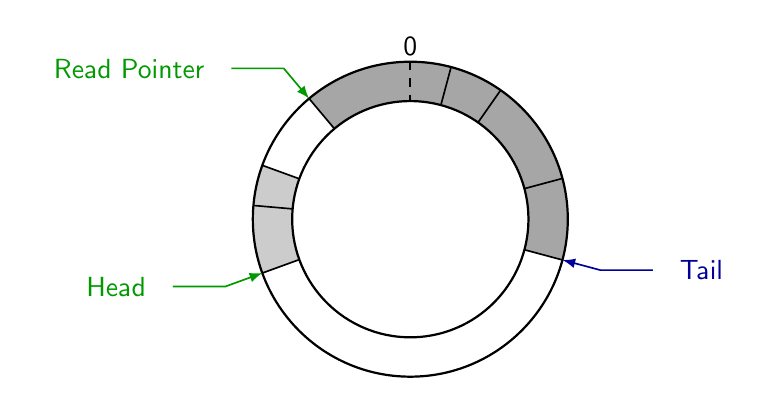
\begin{tikzpicture}[>=latex,font=\sffamily,semithick,scale=2]
    \fill [black!35] (0,0) -- (130:1) arc [end angle=-15, start angle=130, radius=1] -- cycle;

    \fill [black!20] (0,0) -- (200:1) arc [end angle=160, start angle=200, radius=1] -- cycle;
    \draw [thick] (0,0) circle (1cm);

    \node (zero) at (90:1.1) {0};
    \draw[dashed] (90:1) -- (0:0);
    \draw (200:1) -- (0:0);
    \draw (175:1) -- (0:0);
    \draw (160:1) -- (0:0);

    \draw (130:1) -- (0:0);
    \draw (75:1) -- (0:0);
    \draw (55:1) -- (0:0);
    \draw (15:1) -- (0:0);
    \draw (-15:1) -- (0:0);
    \node [circle,thick,fill=white,draw=black,align=center,minimum size=3cm] at (0,0) {};


    \draw [<-,black!40!green] (130:1) -- (130:1.25) -- +(-.333,0)
        node [black!40!green,left,inner xsep=.333cm] (rptr) {Read Pointer};
    \draw [<-,black!40!green] (200:1) -- (200:1.25) -- +(-.333,0)
        node [black!40!green,left,inner xsep=.333cm] (Head) {Head};
    \draw [<-,black!40!blue] (-15:1) -- (-15:1.25) -- +(.333,0)
        node [black!40!blue,right,inner xsep=.333cm] (Tail) {Tail};
\end{tikzpicture}

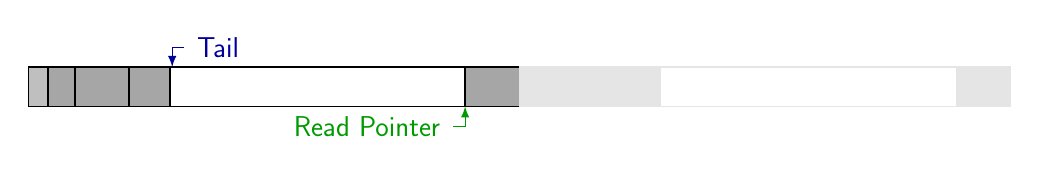
\begin{tikzpicture}[>=latex,font=\sffamily,every node/.style={minimum width=1cm,minimum height=1cm,outer sep=0pt,draw=black,semithick, scale=0.5}]
        \node [minimum width=.5cm, fill=black!25] at (0,0) (A) {};
        \node [anchor=west, minimum width=.68cm, fill=black!35] at (A.east) (B) {};
        \node [anchor=west, minimum width=1.38cm, fill=black!35] at (B.east) (C) {};
        \node [anchor=west, minimum width=1.03cm, fill=black!35] at (C.east) (D) {};
        \node [anchor=west, minimum width=7.5cm] at (D.east) (E) {};

        \node [anchor=west, minimum width=1.38cm, fill=black!35] at (E.east) (F) {};

        \node [anchor=west, minimum width=.5cm, fill=black!10, draw=none] at (F.east) (A') {};
        \node [anchor=west, minimum width=.68cm, fill=black!10, draw=none] at (A'.east) (B') {};
        \node [anchor=west, minimum width=1.38cm, fill=black!10, draw=none] at (B'.east) (C') {};
        \node [anchor=west, minimum width=1.03cm, fill=black!10, draw=none] at (C'.east) (D') {};
        \node [anchor=west, minimum width=7.5cm, draw=none] at (D'.east) (E') {};
        \node [anchor=west, minimum width=1.38cm, fill=black!10, draw=none] at (E'.east) (F') {};
        \node [anchor=west, minimum width=12.47cm, draw=black!10] at (F.east) (A') {};

        \draw [<-,black!40!blue, scale=1] (1.7,.25) -- (1.7, .5)  -- +(.15,0)
        node [black!40!blue,right,inner xsep=.333cm, draw=none] (Tail) {\huge Tail};
        \draw [<-,black!40!green, scale=1] (5.42,-.25) -- +(0, -.25)  -- +(-.15,-.25)
        node [black!40!green,left,inner xsep=.333cm, draw=none] (Head) {\huge Read Pointer};

\end{tikzpicture}
\end{center}
\caption{Ring Buffer with twice mapped memory to allows DMA writes over the end}
\comment{Fix figure to include read pointer correctly}
\label{fig:ringbuffer}
\end{figure}

The core of our buffered read connection is a ring buffer. This buffer ensures that the sender always knows \emph{where} to 
write to. Figure \ref{fig:ringbuffer} shows the basis for our ring buffer that we use for all implementations.

\paragraph{} We use a buffer that allows us to write arbitrary message sizes. There are three relevant pointers. 
The \emph{tail} which points to the next free memory address, the \emph{head}, which points to  the end of the 
free memory region, and the \emph{read pointer} which points to the start of the next unprocessed message. 

\paragraph{} The tail is only stored and updated by the sender. The tail directly gives the sender the address to write the 
next message to. The only thing the sender needs to check is, if there is actually enough space in the buffer for the 
intended message. So it needs at least a semi regular update on the head position. We look into this problem in 
the \emph{Acknowledging} section below.

\paragraph{} Receiving is a little more involved. Similarly to how we implemented the receive buffer management in 
Section \ref{sec:conn:send} we want to have the notion of \emph{reading} which returns a pointer to the start of 
the next unread message and \emph{freeing} a message which allows us to reuse that section of the ring buffer. 

This is where the difference between the \emph{head} and the \emph{read pointer} becomes apparent. The read pointer points 
to the next message the receiver has not read, while the head points to the oldest message the receiver has not freed. Reading
and freeing messages should work while interleaving, so we need some kind of management of free buffer to update the head 
correctly.

We solve this in a very simple way by having a linked list containing the starting address of the received messages. When
reading we push the address to the end of the list. When freeing we remove it from the list. The head is always the first 
element in the list.

We should note that the length of the message has to be communicated in some way, which we will address in the section 
\emph{Sending} below.





\paragraph{"Magic" Buffer} One problem we encountered while using such a ring buffer for RDMA is that we cannot simply 
\emph{wrap around} the end of the buffer using DMA. So if we want to write a message that is larger then the space left until
the end of the buffer we either need to skip to the front of the buffer, wasting space, or perform two writes, which is 
significantly slower.

Figure \ref{fig:ringbuffer} shows the our problem. Message $A$ cannot be written in a single RDMA write as it consists of 
two distinct, not connected memory regions. We can solve this by using something that has been coined 
\emph{"Magic" ring buffer} \comment{By? rgiesen.wordpress.com? Someone else?}. The idea is to map the same physical twice,
so that the same physical memory is adjacent to itself in virtual memory. You can see a representation of this in the 
Figure above. We use \emph{shared memory segments} on Linux to achieve this memory layout.

With this change we can simply write over the end of the buffer and do not have to worry about wrapping around.

\subsubsection{Sending}
With the ring buffer described above, the sender always knows where to write the next message to. We still need to solve
the problem of notifying the receiver that we sent a message and communicate the size of this message.

\paragraph{}The sender and receiver interfaces stay exactly the same as presented in Section \ref{sec:conn:send}. We use the same 
monotonically increasing \code{wr\_id}s to wait for sends to complete. The freeing is explained in the buffer section
above. We implemented three different ways to send and receive


\paragraph{Write Immediate}

We introduced \emph{Write with Immediate} in Section \ref{sec:bg:write}, which basically allows us to implement our sending 
and receiving in a very similar way to the send connection presented in the last section.

\paragraph{} Write with Immediate sends a 32 bit value while also writing to the specified location. More importantly it 
consumes a receive buffer and creates a completion event at the receiver. This completion event also contains the number 
of bytes written. So by writing the message using write with immediate, we will generate a completion event at the receiver
which gives it the size of the message. The receiver can then immediately repost the received buffer and return the ring 
buffer segment. Through the in order guarantees of RDMA we know that the messages in the ring buffer will be in the same
order as the completion events in the queue. We can reuse both the receive buffer management and batching from the send 
connection.


\paragraph{Write Offset}

One key reason to use the write instead of send verb is that we do not need to generate a completion event at the receiver
and the common knowledge that writes are faster than sends~\cite{}\comment{Cite some papers that say this}. When we use 
write with immediate however, we expect the same performance as when using the send verb and we still need to handle receive
buffers and completion events. So we need other ways to notify the sender of incoming messages.

\paragraph{} One way to implement this is by having additional metadata that allows the receiver to notice incoming data.
We implement such a protocol with what we call \emph{Write Offset}. The idea is that together with each message, the sender
also updates a metadata region at the receiver containing the \emph{tail}. The receive can then notice new incoming messages
by polling this tail and comparing it to the \emph{Read Pointer}. We solve the problem of finding the size of the messages by
writing it in the first 4 bytes of the written segment.

\paragraph{} This means to send a message of size $s$ the sender prepends the size $s$ to the message and writes it to the
tail of the buffer. It then writes the updated tail to the metadata region at the sender. Of these two RDMA writes only the 
latter needs to be signaled and we can issue both of the work requests at the same time, mitigating the impact of having to 
perform two writes for a single message. The receiver will always poll its local copy of the tail. As soon as the tail does 
not equal it \emph{Read Pointer} it knows that there are outstanding messages. We can read the first 4 bytes to get the size
of the next message and can then read it and update the \emph{Read Pointer}.

\paragraph{} This connection has obvious drawbacks, as we need to issue two writes for a single message. But this way we 
circumvent the need of receive buffers and end up with a completely \emph{passive receiver}. We thought of other metadata
based implementations of buffered read. For example instead of pushing the tail update to the receiver with each write, the
receiver could actively pull the tail update using RDMA read when necessary. This could potentially outperform the push based
implementation in high bandwidth situations. We did however not implement and evaluate this pull based approach.


\paragraph{Write Reverse}

With our \emph{Write Reverse} connection implementation we are able to notify the receiver without an additional write or
consuming a receive buffer. We can do this by polling on the actual transmitted data. Previous work~\cite{herd, farm} has
shown that RDMA updates memory in increasing memory order, at least for any modern systems we know. This allows us to poll
on the highest memory address to check whether a transfer is complete.

\begin{figure}[!hb]
\begin{center}

\begin{tikzpicture}[>=latex,font=\sffamily,semithick,scale=2]
  \draw [draw=none, fill=black!20] (20:2) arc [end angle=95, start angle=20, radius=2] -- (95:1.75)  arc [end angle=20, start angle=95, radius=1.75] -- cycle;
  \draw [draw=none, fill=green!10] (95:2) arc [end angle=145, start angle=95, radius=2] -- (145:1.75)  arc [end angle=95, start angle=145, radius=1.75] -- cycle;
  \draw (160:2) arc [end angle=20, start angle=160, radius=2];
  \draw (160:1.75) arc [end angle=20, start angle=160, radius=1.75];

  \draw (145:2) -- (145:1.75);
  \draw (140:2) -- (140:1.75);
  \draw[decoration={
            text along path,
            text={0},
            text align={center},
            raise=0.15cm},decorate] (145:1.75) arc (145:140:1.75);
  \draw (100:2) -- (100:1.75);
  \draw[decoration={
            text along path,
            text={data},
            text align={center},
            raise=0.15cm},decorate] (140:1.75) arc (140:100:1.75);


  \draw (95:2)  -- (95:1.75);
  \draw[decoration={
            text along path,
            text={1},
            text align={center},
            raise=0.15cm},decorate] (100:1.75) arc (100:95:1.75);

  \draw [<-,black!40!blue] (95:2) -- (95:2.25) 
        node [black!40!blue,above,inner xsep=.333cm] (Tail) {Tail};

  \draw [<-,black!20!blue] (140:2) -- (140:2.25) 
        node [black!20!blue,above,inner xsep=.333cm] (ntail) {\small New Tail};



  \draw (60:2)  -- (60:1.75);
  \draw (55:2)  -- (55:1.75);

\end{tikzpicture}
\end{center}
\caption{Reversed Ring buffer}
\label{fig:write-rev}
\end{figure}

\paragraph{} So the core idea is to append a \emph{valid byte} at the end of the message on which the receiver can poll on.
There are two issues with introducing this two our existing ring buffer design.

\begin{itemize}
  \item The messages have variable size, so the receive does not know the location of this \emph{valid byte}.
  \item We need to zero this byte after freeing the buffer segment, potentially forcing us to zero the complete segment 
    which is fairly expensive.
\end{itemize}

We can solve both these problems by flipping our ring buffer. Instead of writing in increasing order, we add messages in 
decreasing order. Figure \ref{fig:write-rev} shows how writing a message works, the newly written message is highlighted in 
light green. We write a message structure of: 
A zero byte, followed by the data, the message length, and a valid byte, which is set to one. This has the effect that the
receiver can poll on the next byte in the ring buffer to check for new incoming messages and read the next 4 bytes to get 
the size of it. The prepended zero byte actually zeros the valid byte of the next massage. This means the receiver does not 
need to zero anything after freeing the segment.




We note that reversing the ring buffer does not really change any implementation details presented in 
Section~\ref{sec:conn:write:buf}. The double mapped memory trick still works and the freeing of buffers still works in a
similar way.

\subsubsection{Acknowledging}

We showed that there are multiple ways to transfer data and notify the sender. One other thing we need to prevent is for the
sender to overrun the ring buffer. That means the sender needs at leas a periodic update of the head position to decide if
there is space left to write to. We call this \emph{acknowledging} the head position.

We present two different approaches to do this. A pull based approach, where the sender reads the updated head from the
receiver, and a push based approach, where the receiver sends updates to the sender when the head position changes.

\paragraph{Pull} For the pull based implementation the receiver has a dedicated memory region where it writes the current 
head to. The sender has a cache of this head position. As soon as there is not enough space for the next message, given 
the cached head value, the sender will perform a RDMA read to update its cache.

Our current implementation will immediately block until the read succeeds. There is potential to optimize this by preemptively 
updating the head without waiting for it to complete. We experimented adding this, but as we did not see any significant 
performance improvements by adding this, we decided not to add this to reduce complexity. \comment{Maybe we should add it. Its ready}

\paragraph{Push} We also implemented a push based approach, where the receiver will send updates of the tail value using 
RDMA sends. To reduce the load of this acknowledgements we only send updates when the receiver has processed an eighth of 
the complete ring buffer. The sender will then poll its receive queue as soon as it cannot write the next message given its
cache of the tail value.

\subsection{Evaluation}
\todo{Info on system etc.}

\subsubsection{Latency}

\begin{figure}[h]
\includegraphics[width=1\textwidth]{write-lat-msgsize.png}
\caption{Evaluation of the Send Receive latency between two nodes and our performance model}
\label{fig:plot-write-lat}
\end{figure}

Figure \ref{fig:plot-write-lat} shows the latency the latency of sending a message of varying sizes using our write protocol
with all presented sender. All measurements use the \emph{read} acknowledger. There is no significant difference in latency
when switching to a \emph{send} acknowledger. \todo{do we need a graph for that?}
We again perform \emph{ping-pong} measurements. We take half of this RTT as our measurement of latency.


We can see that the additionally issued write of the \emph{WriteOff} gives us a noticeable increase in latency for all message
sizes. The overhead however does seem to decrease a little for messages over the MTU of $4096$ Bytes. This is something we are
not quite able to predict with our model. \todo{Why?}

The latency characteristics of \emph{WriteRev} and \emph{WriteImm} seem to be very similar. This is in line with what we expect
..

\subsubsection{Bandwidth}

\begin{figure}[h]
\includegraphics[width=1\textwidth]{write-bw-unack.png}
\caption{Evaluation of the Send Receive latency between two nodes and our performance model}
\label{fig:plot-write-bw-unack}
\end{figure}

For us to be able to \todo{Something Something full pipeline. Should we really include this graphic}. For the send protocol 
we did not implement any sender side batching. We did show that sender site batching is effective and can have its uses in 
Section \ref{sendrcv}, but application level batching is in the end more effective when possible, so we decided not to look 
into batching for the remaining protocols. We would however expect similar improvements for the buffered write 
protocols with batching.









\pagebreak
\subsection{Shared Write}
\todo{Write Atomic}
\subsubsection{Design}
\todo{Description of the connection and base performance model for latency and bandwidth}
\subsubsection{Device Memory}
\todo{Introduce device memory, show microbench and update performance model}
\subsubsection{Evaluation}

\pagebreak
\subsection{Direct Write}
\todo{Write Write}
\subsubsection{Design}
\todo{Description of the connection and base performance model for latency and bandwidth}
\subsubsection{Send Comparison}
\todo{How does this differ from send receive. No completion queue event}
\subsubsection{Evaluation}
\todo{Maybe already compare to send receive performance}

\pagebreak

\section{Buffered Read}
\subsection{Design}

\begin{figure}[!ht]
\begin{center}
\begin{tikzpicture}[node distance=2cm,auto,>=stealth']
  \seqnode{B_cpu}{RAM};
  \seqnode[left of=B_cpu]{B_nic}{NIC};
  \hseqnode[right of=B_cpu, node distance=1.5cm]{B_acpu}{};
  \seqnode[left of=B_cpu, node distance=7cm]{A_cpu}{CPU / RAM};
  \seqnode[right of=A_cpu]{A_nic}{NIC};
  %
  \msg{B_acpu}{B_nic}{.15}{read WR MMIO}
  \msg{B_nic}{A_nic}{.2}{transfer read request}
  \msg{A_cpu}{A_nic}{.3}{meta DMA}
  \msg{A_nic}{B_nic}{.35}{transfer meta}
  \msg{B_nic}{B_cpu}{.4}{meta DMA}
  \msg[below]{B_nic}{B_cpu}{.45}{WQE DMA}
  \fetch{B_acpu}{B_cpu}{.5}{poll CQ}

  \msg{B_acpu}{B_nic}{.6}{read WR MMIO}
  \msg{B_nic}{A_nic}{.65}{transfer read request}
  \msg{A_cpu}{A_nic}{.75}{payload DMA}
  \msg{A_nic}{B_nic}{.8}{transfer payload}
  \msg{B_nic}{B_cpu}{.9}{payload DMA}
  \msg[below]{B_nic}{B_cpu}{.95}{WQE DMA}
  \fetch{B_acpu}{B_cpu}{1}{poll CQ}

  \end{tikzpicture}
\end{center}
\caption{Buffered Read sequence}
\label{fig:seq-buf-read}
\end{figure}

\todo{This is actually worse when there is no message ready. If the sender updates the head just at the most inoppertune moment
we would waste a whole meta read request}

\subsection{Evaluation}


\pagebreak

\section{Direct Read} \label{sec:conn:direct_read}
\subsection{Design}

In Section~\ref{sec:conn:direct_write} we discussed how we can possibly avoid an additional copy at the receiver by giving 
the sender information which allows him to potentially write the data to the correct final memory location. The next logical
step is to let the receiver decide for each message where to write it to. We can achieve this by our implementation of a
\emph{Direct Read Connection}.

\paragraph{} The core idea of a direct read protocol is that instead of directly sending a message through a send or write 
verb, the sender simply notifies the receiver of a new message and where it is located, we will call this a \emph{Read Request}.
The receiver then issues an RDMA read operation to directly read this message to the correct location.

By allowing to sender to attach additional domain specific information to this read request, the receiver can directly 
move this data to the correct space in a data structure, or potentially even directly NVMe storage for certain applications.
\comment{I remember correctly this is possible right? I had a hard time finding a relevant paper}


\subsubsection{Sender}
The sender interface is again largely unchanged and consists of a \code{SendAsync()} method which takes a buffer containing the
message and a \code{Wait()} method that waits until the transfer is completed.

\paragraph{} Instead of sending the complete buffer, the sender only sends a small \emph{Read Request} using an inline send,
containing the location of the buffer. It is then the job of the receiver to access this buffer.

\paragraph{} To wait for the transfer to be completed, and for the buffer to be able to be reused, we can not simply wait 
for the completion event of the send, like we do for the send or write based connections. We need to wait for the receiver 
to explicitly signal that the buffer was transfered. We append a signaling byte at the end of the sending buffer. 
When sending this byte will be set to 0 and we can wait for the transport to be completed by polling this byte until the 
receiver will update it.

This push based implementation introduces little additional complexity, but there are many different ways to implement such 
signaling. The signaling bit forces us to use a specific memory arrangement, which could prevent us to send data directly 
from certain data structures. In such cases a pull based approach or an implementation using send might be a better approach
and depending on the implementation could actually result in better performance.

\subsubsection{Receiver}
The receiver polls the receive queue and receive the \emph{Read Request}. It then instantly reposts the associated 
receive buffer. With this information it then issues a read request for the message. As for this connection the receiver is
doing the heavy lifting, it is crucial that we do not block until the read is completed to get reasonable performance. 

\paragraph{} This means the receiver has a slightly different interface that the previously presented connections. 
We split the receive call into a \code{RequestAsync} and a \code{Wait} method. The \code{RequestAsync} takes a receive buffer
to read into. It will wait for an incoming read request and issue the corresponding read. It uses the same increasing 
\code{wr\_id} approach we use for sending with which the \code{Wait} method can wait for the read to complete. This approach
allows us to pipeline receives the same way we pipeline sends.

\paragraph{} To update the signal byte to notify the that the transfer is complete we implement to different approaches.

Our first approach is to issue the write with the update at the same time as we issue the read. This however introduces a 
problem. While RDMA guarantees that two consecutive will happen in the issued order, it will not guarantee us that reads issued
before writes will be completed before we can observe the write~\cite{}. \comment{I think we need some kind of references for
that} To still be able to issue these two operations at the same time, we need to use a \code{IBV\_SEND\_FENCE}. When we add 
fence indicator to a write request its processing will not begin until all previous read and atomic operations on the same QP 
have completed. This allows us to issue both the read as well as the acknowledging write at the same time.

The other approach is simply to wait for the read to be completed before issuing the acknowledging write. In other words the
write will be posted as soon as \code{Wait} returns. That way we can avoid the fence which can be quite expensive.

\subsection{Evaluation}


\begin{align*}
  t_{dr} &\geq o_{rr} + o_{rd} + (k-1)G + L  + o_{rcv} + o_{cq}\\
         &\geq o_{sil} + o_{snd} + 3L  + (k-1)G  + 2o_{rcv} + 2o_{cq}
\end{align*}


\begin{figure}[h]
\includegraphics[width=1\textwidth]{dir-read-lat-msgsize.png}
\label{fig:plot-dirread-lat}
\end{figure}


\begin{figure}[h]
\includegraphics[width=1\textwidth]{dir-read-bw-msgsize.png}
\label{fig:plot-dirread-bw}
\end{figure}



\begin{figure}[h]
\includegraphics[width=1\textwidth]{dir-read-bw-threads.png}
\label{fig:plot-dirread-bw-threads}
\end{figure}


\begin{figure}[h]
\includegraphics[width=1\textwidth]{dir-read-bw-n1.png}
\label{fig:plot-dirread-bw-n1}
\end{figure}



\pagebreak
\section{Comparison}
\todo{Comparison between connection types. Show which protocols perform better in which sitations.}

\subsection{Point to Point - N:N}

\subsection{Server Model - N:1}

\subsection{Fan Out / Broadcast - 1:N}

\pagebreak
\section{Conclusion}



\pagebreak

\bibliographystyle{unsrt}
\bibliography{references}{}

\end{document}
